 \section{Methodology}\label{sec:meth}
 \subsection{Resonance Equalization}\label{sec:re}
 State-variable-feedback (SVF) is a control method that uses different states of a system, such as position,
velocity, and acceleration, to create an input to achieve a desired performance. In this case the states of the
system consist of the angular position, angular velocity, and angular acceleration with the input being
torque. At this point it is pertinent to note the torque applied by a direct current (DC) motor is directly
proportional to the current through the windings of the motor. It is also pertinent to note that it is widely
known that the DC motor is a fully observable system when the output is the angular position, thus a full or
partial state observer can be made for this system. With the latter being said Rizzo et. al.\cite{bigley1978resonance}
analyzed what the effects of TR had on various parameters of the system including shaft velocity and input
current, Fig.~\ref{fig:re} is an example of some of these plots.  A key point noted is that the input current and output velocity are
almost exactly $180^o$ out of phase from one another. The importance of this is that the actuator shaft
velocity can be used as feedback in combination with the input current to compensate for the effects of the 
resonance. The latter relationship will ensure that the control is effective for changes in the resonant
frequencies.

\begin{figure}[t]
  \centering
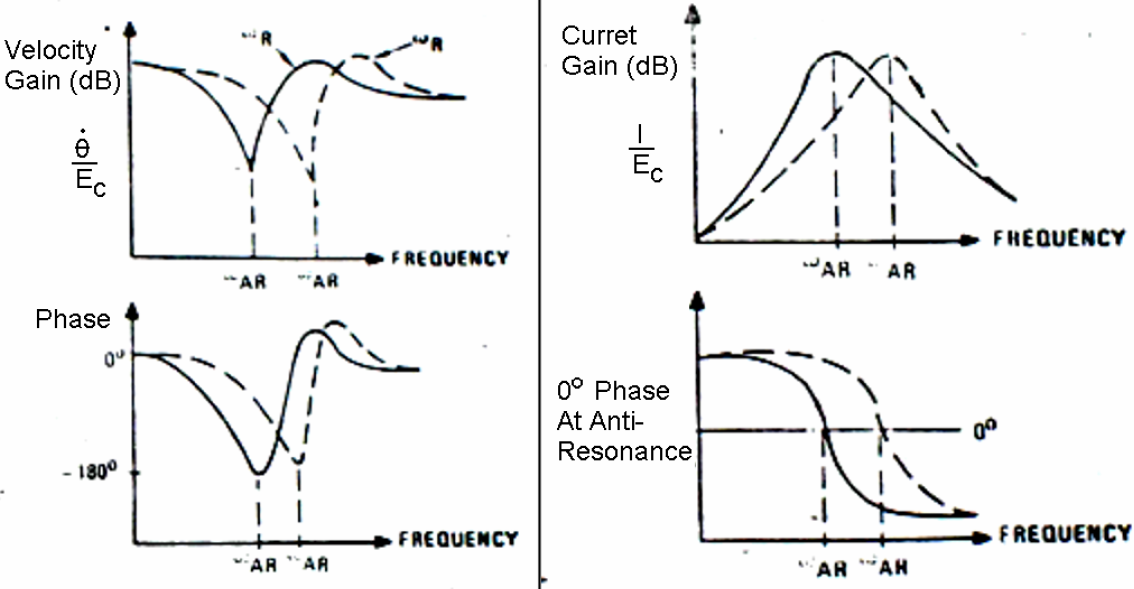
\includegraphics[width=1.0\columnwidth]{./pix/re.png}
  \caption{Plot of the Actuator Shaft Velocity and Phase (Left), Plot of the Actuator Current and
Phase (Right) around $\omega_r$ and $\omega_{ar}$\cite{bigley1978resonance}}
  \label{fig:re}
\end{figure}

Using the knowledge that the current, or torque, is about $180^o$ out of phase with the angular velocity of
the actuator Rizzo showed that ``\textit{the resonance peaking factor F is completely
eliminated}.'' Rizzo�s method is implemented in Fig.~\ref{fig:reSim} with the SVF gains of -0.2 for the current
feedback gain and 20 for the angular velocity feedback. Table~\ref{table:resultsClosedLoop} shows the maximum change 
in magnitude and phase of the frequency response plot of the
system with TR and the addition of Rizzo�s resonance equalization (RE)\cite{bigley1978resonance}.

\begin{figure}[ht]
  \centering
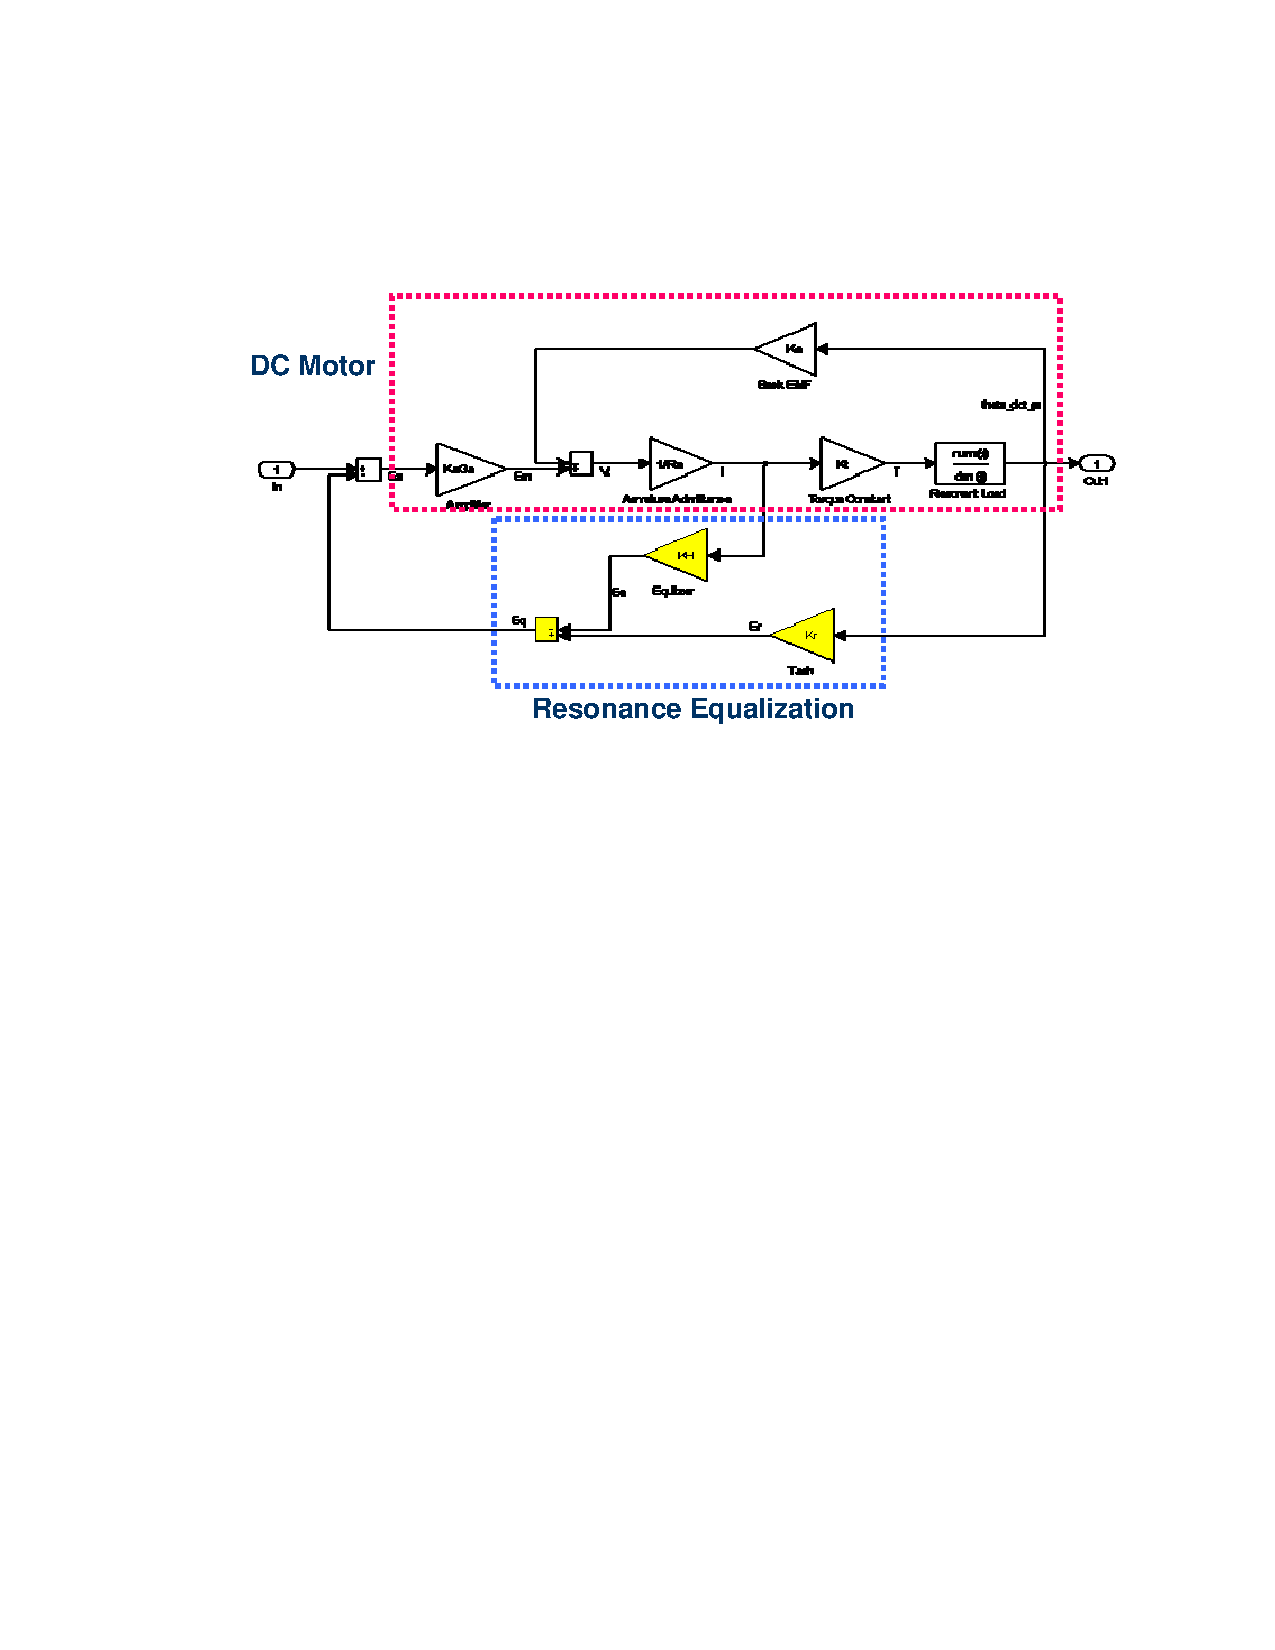
\includegraphics[width=1.0\columnwidth]{./pix/reSim.pdf}
  \caption{V.Rizzo�s resonance equalized rate loop diagram using SVF\cite{bigley1978resonance}}
  \label{fig:reSim}
\end{figure}


This results in a reduction of the resonance and anti-resonance and the corresponding phase shift.  Fig.~\ref{fig:reBode} shows the frequency response of RE on the TR system.  RE eliminates the load switching ($\Delta dB$) as shown in Fig.~\ref{fig:trBode}.  However the motor velocity $\dot{\theta_a}$ and motor current $i_a$ states are required to implement RE.

\begin{figure}[ht]
  \centering
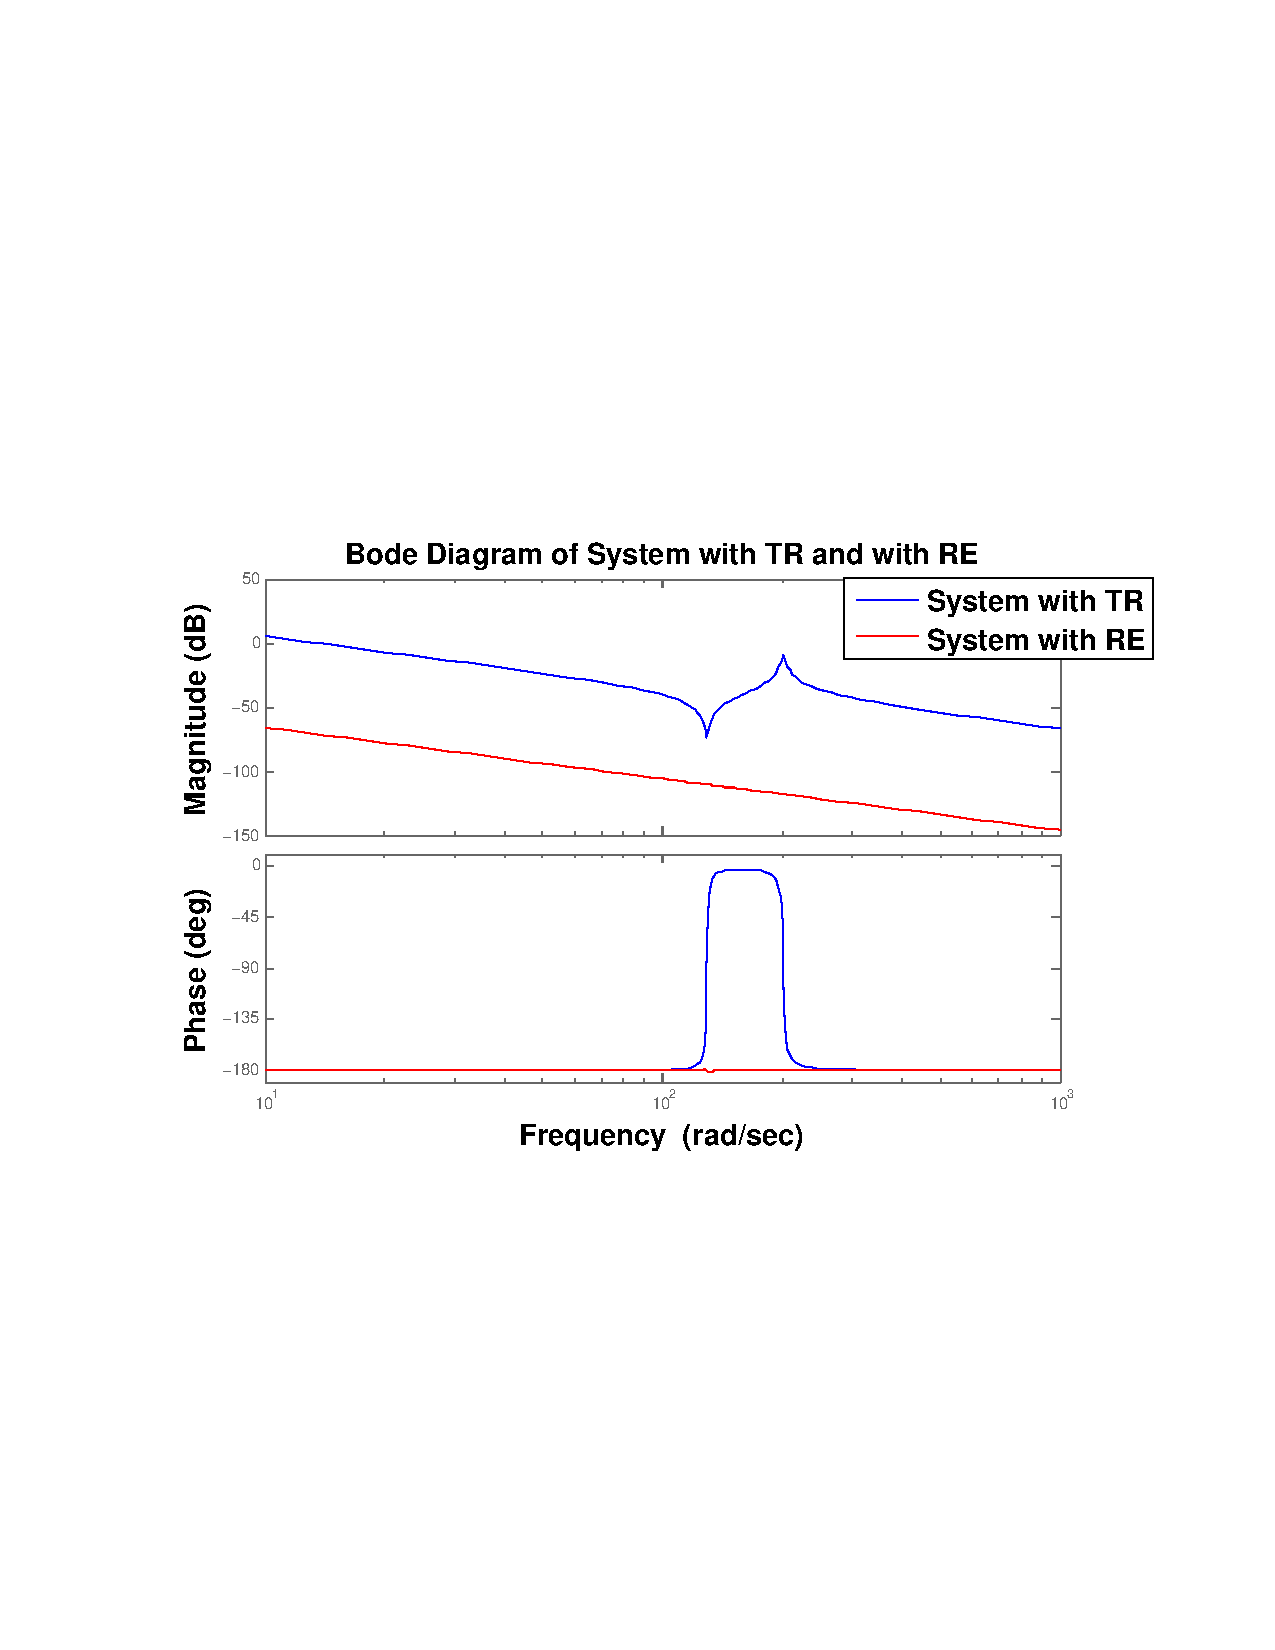
\includegraphics[width=1\columnwidth]{./pix/bodeTRandRE4.pdf}
  \caption{Frequency response of V. Rizzo�s resonance equalization (RED) plotted over a system exhibiting TR system (BLUE).  The resonance equalized system is using an ideal model of a DC motor for use in the state variable feedback.}
  \label{fig:reBode}
\end{figure}


\subsection{Sliding Mode Control}\label{sec:smc}
Sliding Mode Control (SMC) is a form of non-linear control that is able deal with systems that are not
linear as well as systems that have parameters which are not precisely known. 
We are using sliding mode with boundary layer as defined in Slotine et. al\cite{slotine}.  
This leads to tracking within a guaranteed precision $\epsilon$ (rather than perfect tracking) and generally guarantees that for all trajectories starting inside boundary layer $\mbox{B}$ (see Fig~\ref{fig:smcSliding})  where 

\begin{equation}
\begin{array}{ccc}
\mbox{B} = \{ x , \left| s(x;t) \right|  <=  \Phi \}
&  
\mbox{where}
&
\Phi > 0
\end{array}
\end{equation}


When using SMC one, or multiple, parameters are chosen to be unknown. 
These unknown parameters are specified a range at which the given parameters are able to vary between and retain system perform within its given bounds $\psi$ and $\epsilon$. 
It is important to note that this range affects the boundary condition $\psi$ and $\epsilon$. Once the system has entered within the boundary layer, or sliding boundary, it will not leave it. 
The latter will hold true as long as the parameters which are able to vary do not go out
of the designed bounds \cite{kwatny2000nonlinear}\cite{isidori1995nonlinear}.


\begin{figure}[h]
  \centering
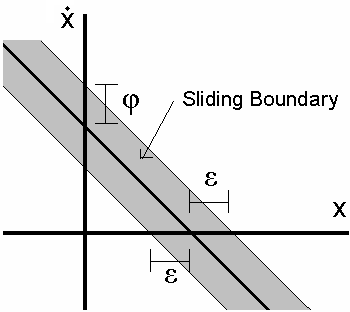
\includegraphics[width=0.7\columnwidth]{./pix/smc2.png}
  \caption{SMC Sliding Boundary/Sliding Layer $\mbox{B}$}
  \label{fig:smcSliding}
\end{figure}

The fact that a parameter can be defined to be between a given bound and still have stable control is one of
SMC�s strongest arguments for it�s use for the the reduction of TR. This is also because an exact model of
the system does not have to be made for SMC to be effective. SMC is able to take care of some of the unmodeled
dynamics including TR. Fig.~\ref{fig:trBode} shows the effective inertial load on a system with TR before $\omega_{ar}$
and after $\omega_r$. As stated previously in Fig.~\ref{fig:trBode} and Eq.~\ref{eq:deltaDB} there is an offset in the magnitude of the
frequency response due to the change in the effective load. Due to the latter the inertia has been chosen to
be the parameter to be unknown within a given bound. The inertial load will vary from $0.9J_a$ to $1.1(J_a+J_L)$
to ensure the system will always fall within the bounds of the SMC and thus stay within the sliding
boundary.

The effective load has been taken care of by letting it vary; thus the model of the TR system from Fig.~\ref{fig:couple} can be reduced and assumed to be a system with out TR, see Fig.~\ref{fig:smcSliding}.

\begin{figure}[h]
  \centering
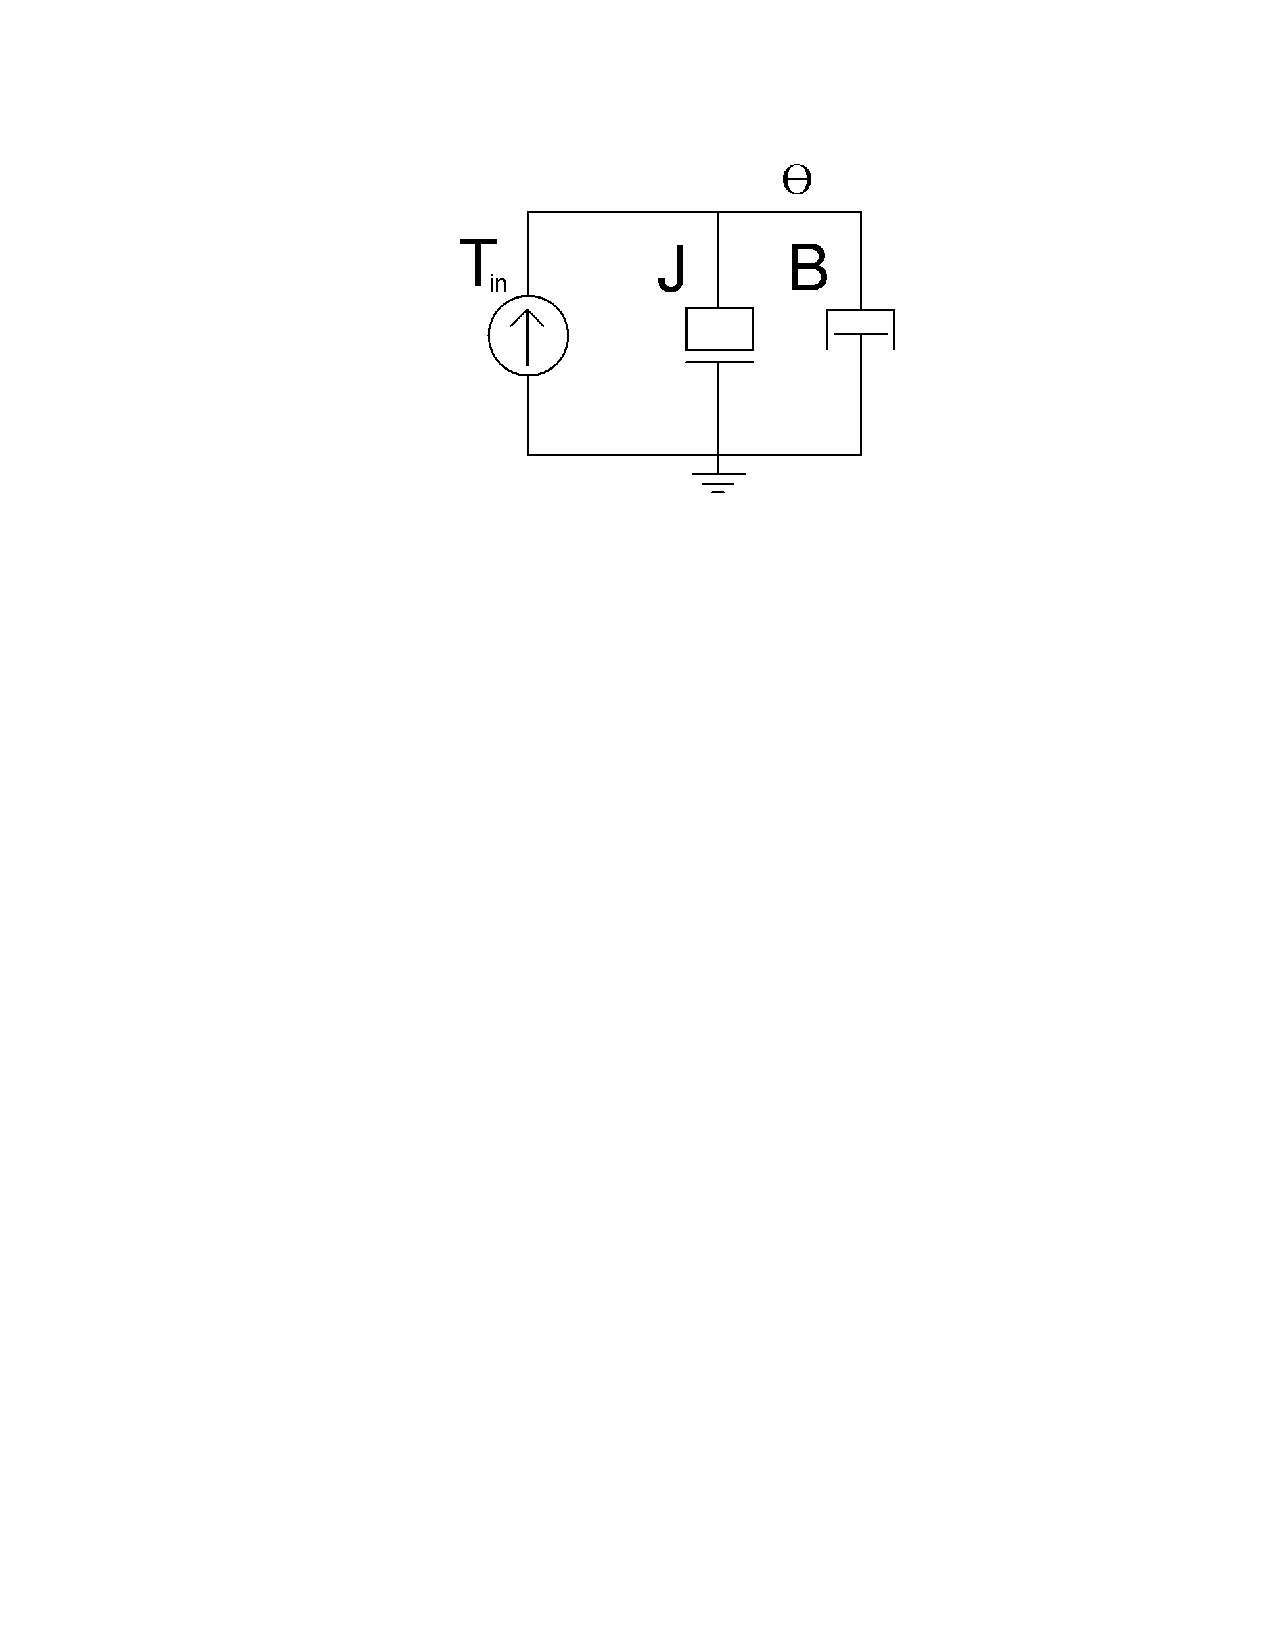
\includegraphics[width=0.7\columnwidth]{./pix/smcMech.pdf}
  \caption{Mechanical Schematic Drawling of Reduced System for SMC based on Fig~\ref{fig:couple}}
  \label{fig:smcMech}
\end{figure}

\noindent The dynamic equations for the system in Fig.~\ref{fig:smcSliding} are written as

\begin{equation}
\begin{array}{ccc}
T(t) = J\ddot{\theta}+B\dot{\theta} & \rightarrow & \ddot{\theta} = \frac{1}{J}T(t) - \frac{B}{J}\dot{\theta}
\end{array}
\end{equation}


\noindent to implement the SMC $u$ that consists of the approximation of continuous control $\hat{u}$ combined with a switching mode $Q\mbox{sgn}(r)$ that is designed to keep the system on the sliding surface

\begin{equation}
u = \hat{u}-Q\mbox{sgn}(r)
\end{equation}

\noindent where $r$ is the sliding surface

\begin{equation}
r = \dot{\tilde{\theta}} + \lambda \tilde{\theta}
\end{equation}

\noindent and

\begin{equation}
\hat{u} = \hat{b}^{-1}\left[\ddot{\theta_d}-\hat{f}-\lambda \dot{\tilde{\theta}}\right]
\end{equation}

\noindent where $d$ denotes the desired state, $\hat{}$ denotes the estimate, $\tilde{}$ denotes the error between the observed state and the desired state, $\lambda$ is a gain chosen on a per-system basis, and the following parameters are defined as

\begin{equation}
\begin{array}{cc}
b=\frac{1}{J}, & R = \frac{B}{J}
\end{array}
\end{equation}

\noindent and

\begin{equation}
\begin{array}{cc}
f=-R\dot{\theta}, & \hat{f}=-R_{ave}\dot{\theta}
\end{array}
\end{equation}


\noindent where bounds on $J$ and $R$ are set as

\begin{equation}
\begin{array}{ccc}
R_{min}\leq R \leq R_{max}, & R_{min} = \frac{B}{J_a+J_L}, & R_{max} = \frac{B}{J_a}
\end{array}
\end{equation}

\noindent The maximum deviation and average value of $R$ is defined by $R_x$ and $R_{ave}$ respectively

\begin{equation}
\begin{array}{cc}
R_{x} = \left|R_{max}-R_{min}\right|, & R_{ave} = \frac{1}{2}\left(R_{max}+R_{min}\right)
\end{array}
\end{equation}

values of $Q$ mus be sufficiently large so that it stays on the sliding surface

\begin{equation}
Q\geq \hat{b}^{-1}\left(\eta-F\right)+\left(\beta-1\right)\left|\hat{u}\right|
\end{equation}

\noindent where

\begin{equation}
\begin{array}{ccc}
F\geq \left|f-\hat{f}\right| & \rightarrow & F=R_x\left|\dot{\theta}\right|
\end{array}
\end{equation}

\noindent and


\begin{equation}
\begin{array}{ccc}
\beta=\left(\frac{b_{max}}{b_{min}}\right)^{\frac{1}{2}}, 	& 	b_{min}= \frac{1}{J_a+J_L}, 	& b_{max} = \frac{1}{J_a}
\end{array}
\end{equation}

\noindent and $\hat{b}$ (the estimate of $b$) is the geometric mean of $b$. 
The values $\eta$ and $\lambda$ are restricted by the sampling rate of the controller. 
Both of the latter values are not to
exceed a numerical value of half the sampling frequency in Hz.
Fig.~\ref{fig:smcBlock} shows the block diagram of the SMC on the TR system.
Fig.~\ref{fig:danBode} shows the frequency response of SMC on the TR system.

\begin{figure}[h]
  \centering
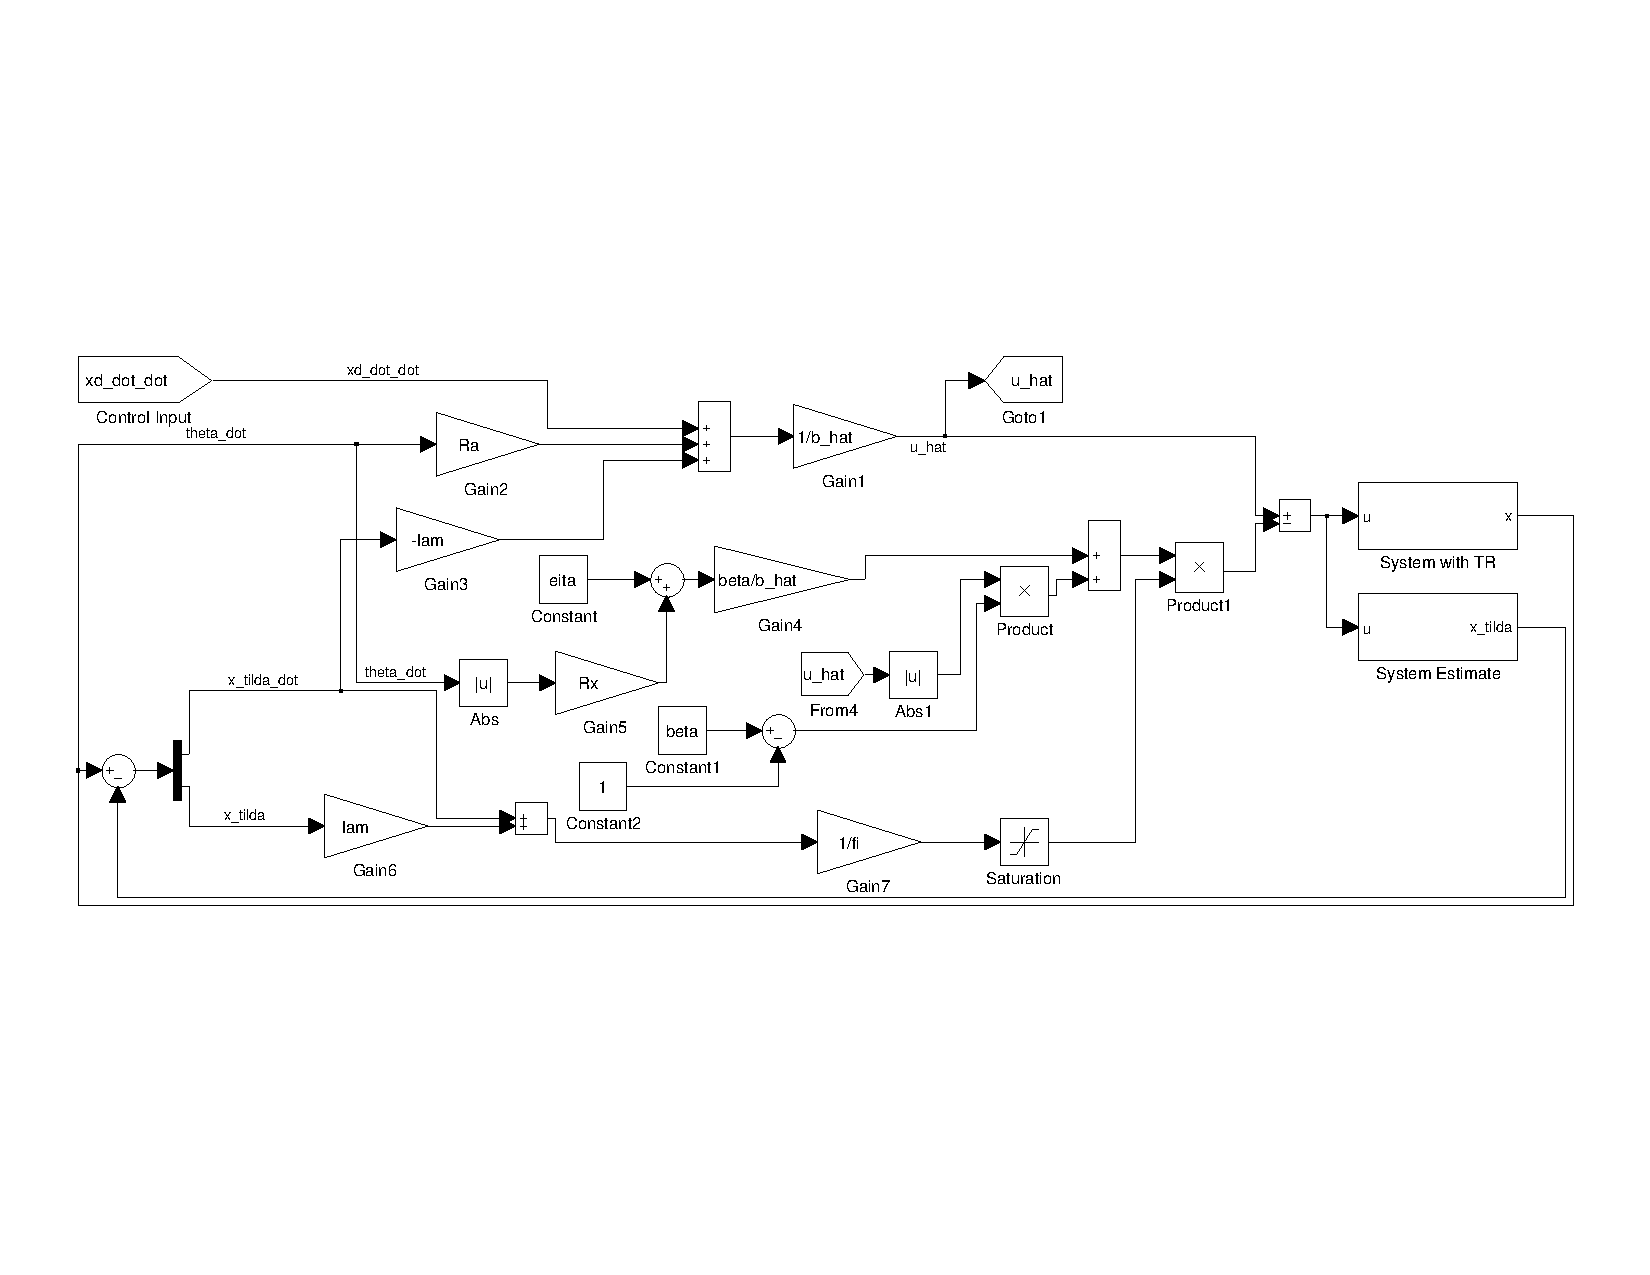
\includegraphics[width=1\columnwidth]{./pix/smcBlock.pdf}
  \caption{Frequency response plot for SMC on system with TR with $\eta= 0.3$ and $\lambda=30,000$}
  \label{fig:danBode}
\end{figure}

Multiple simulations were made on the SMC control method to reduce the effects of TR. Table~\ref{table:resultsClosedLoop} shows the
results of these test for multiple ratios of $J_L:J_a$.  
It is apparent from the simulations that the system will track the desired waveform. 
Load switching has no effect on the system as long as the apparent load stays between $J_{min}$ and $J_{max}$.
As the ration $\frac{J_L}{J_a} \rightarrow 0$ the effect of TR on both the magnitude and the phase goes to zero.
To motor position $\theta_a$ and motor velocity $\dot{\theta}_a$ are needed to preform proper SMC in a TR system. 

%\section{Results}\label{sec:results}


\begin{center}
	\begin{table}
	\caption{Effects of changing the ratio of $J_L:J_a$ (Open Loop) $K_c=55.0\frac{oz}{in}$}
	\begin{center}
  \begin{tabular}{  c | c | c | c }

Ratio					& $J_L$										& $\Delta dB$	& $\Delta$ TR Phase \\ 
($J_L:J_a$)		&($oz\cdot in\cdot sec^2$)& ($dB$)			& ($deg$)							\\	\hline
\hline
2.000  				&0.00460  								&9.542  			&180.0							\\	\hline
1.435  				&0.00330  								&7.729  			&180.0							\\	\hline
0.500  				&0.00115  								&3.522  			&180.0							\\

  \end{tabular}
  \end{center}
  \label{table:resultsOpenLoop}
  \end{table}
\end{center}


\begin{center}
	\begin{table}
	\caption{Effects of changing the ratio of $J_L:J_a$ when using RE and SMC (Closed Loop) $K_c=55.0\frac{oz}{in}$}
	\begin{center}
  \begin{tabular}{ c | c | c | c | c | c }
						&								& 												& 								& $\Delta$ TR 		& $\Delta$ TR 			\\ 
Control			&Ratio					& $J_L$										& $\Delta dB$			& Mag 						& Phase 						\\ 
Method			&($J_L:J_a$)		&($oz\cdot in\cdot sec^2$)& ($dB$)					& ($dB$)					& ($deg$)						\\	\hline
\hline
RE 					&2.000  				&0.00460  								&0.500  					&0.400  					&4.600							\\	\hline
RE 					&1.435  				&0.00330  								&0.300  					&0.200  					&3.500							\\	\hline
RE 					&0.500  				&0.00115  								&0.500  					&0.100  					&1.600							\\	\hline
\hline
SMC 				&2.000  				&0.00460  								&0.000  					&24.652  					&130.840						\\	\hline
SMC 				&1.435  				&0.00330  								&0.000  					&10.200  					&23.770							\\	\hline
SMC 				&0.500  				&0.00115  								&0.000  					&0.012  					&1.815							\\	


  \end{tabular}
  \end{center}
  \label{table:resultsClosedLoop}
  \end{table}
\end{center} 

\begin{figure}[ht]
  \centering
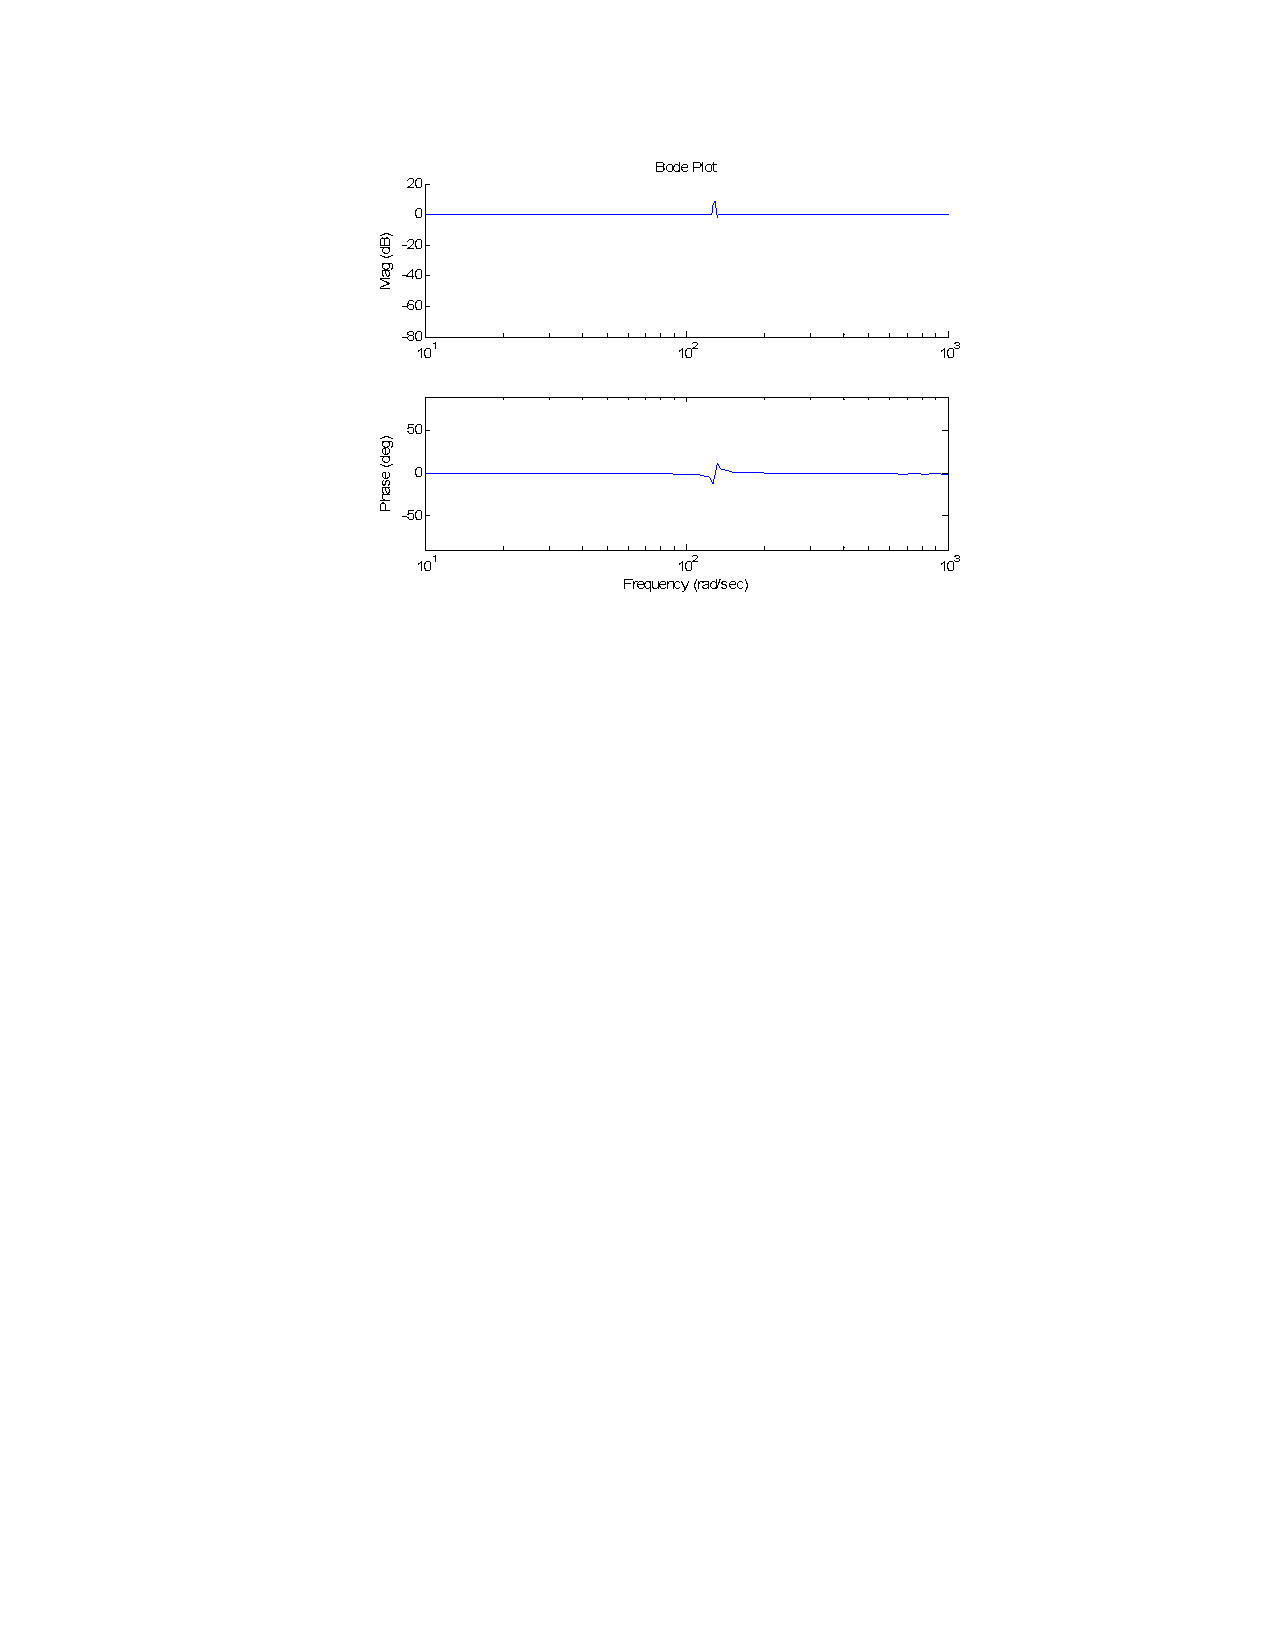
\includegraphics[width=1.0\columnwidth]{./pix/danBode.pdf}
  \caption{Frequency response plot for SMC on system with TR with $\eta= 0.3$ and $\lambda=30,000$}
  \label{fig:danBode}
\end{figure}
